\section{Vorgehen}

Projektorgansation: Organigramm Rollen, Scrum/..., Datenaustausch

Design Thinking, ...

\subsection{Projektorganisation}

Da es sich um eine interdisziplinarische Produktentwicklung handelt, wurde das Team aus jeweils zwei Studierenden aus den Studiengängen \acrfull{elektrotechnik}, \acrfull{informatik} und \acrfull{maschinentechnik} zusammengeführt. In Abbildung \ref{fig:Organigramm} ist die Projektorganisation ersichtlich. 

Im Team wurde Alina Meyer als Projektleiterin gewählt. zudem benötigt es für die Mechanische und Elektrische Werkstetten in der Hochschule Luzern jeweils einen zuständige Person im Team. Welche dem Ivan Zimmerman (\acrshort{elektrotechnik}) und Elias von Atzigen (\acrshort{maschinentechnik}) zugeteilt wurde.

Die klare Aufteilung der Rollen ermöglicht es dem Team, effizient und zielgerichtet an der Entwicklung des Projekts zu arbeiten. Durch diese Struktur wird gewährleistet, dass jede technische Disziplin angemessen abgedeckt ist und die Kommunikation innerhalb des Teams reibungslos funktioniert.

\begin{figure}[h]
\centering
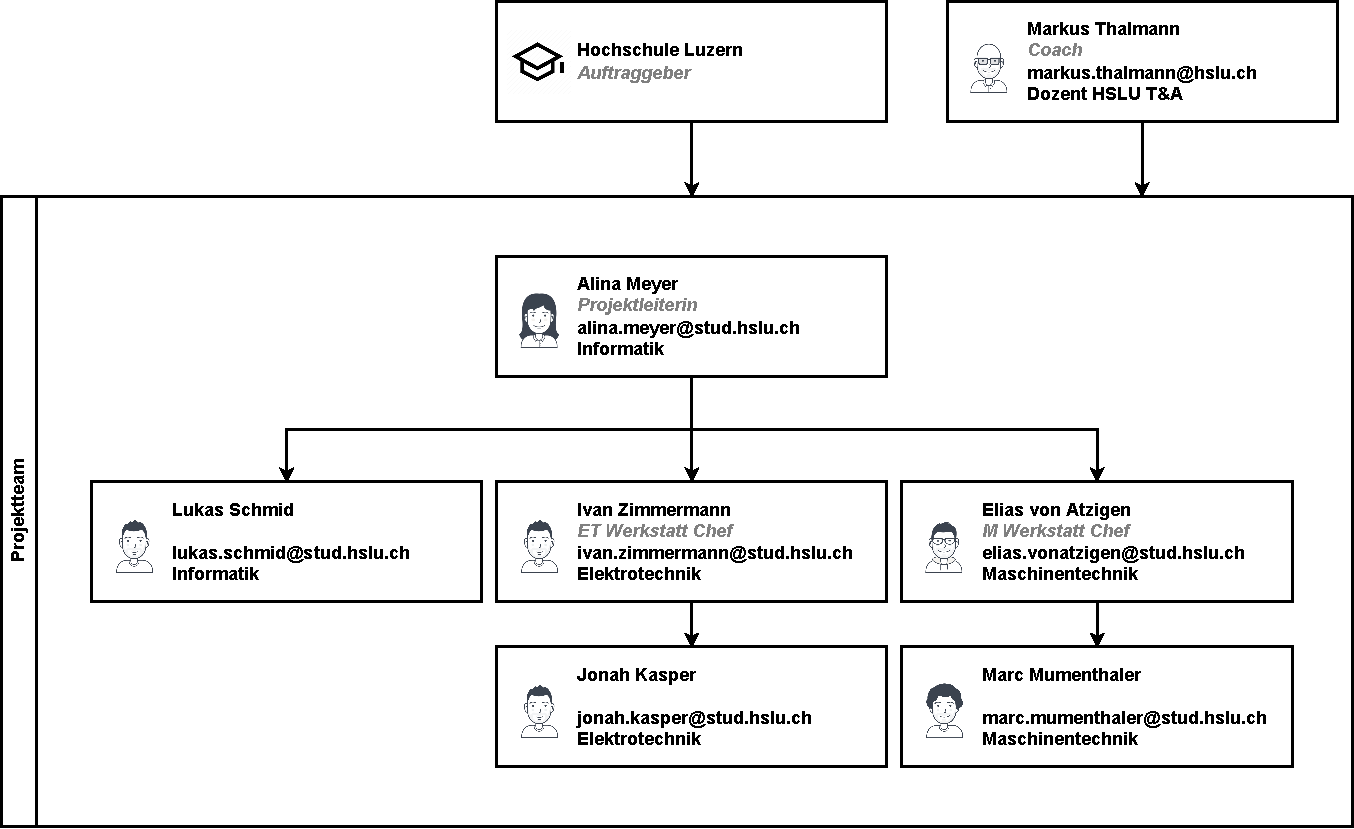
\includegraphics[width=\textwidth]{img/Projektorganisation.pdf}
\caption{Organigramm}
\label{fig:Organigramm}
\end{figure}